\documentclass{standalone}

\usepackage{tikz}
\usetikzlibrary{arrows.meta,angles,quotes}

\usepackage{newtx}
\usepackage{bm}
\renewcommand\mathbf\bm

\begin{document}
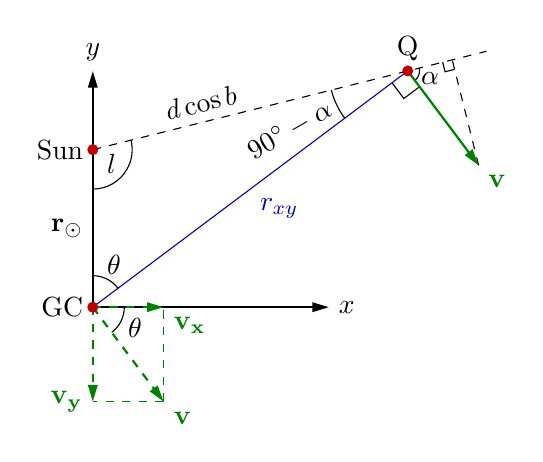
\begin{tikzpicture}
    \coordinate [label=left:GC] (O) at (0,0);
    \coordinate [label=left:Sun] (S) at (0,2);
    \coordinate [label=above:Q] (Q) at (4,3);
    \coordinate [label=below right:\textcolor{green!50!black}{$\mathbf{v}$}] (V) at (4.9,1.8);
    \coordinate [label=above:$y$] (Y) at (0,3);
    \coordinate [label=right:$x$] (X) at (3,0);
    \draw [-{Triangle[length=10pt,scale=0.6]},thick] (O) -- (Y);
    \draw [-{Triangle[length=10pt,scale=0.6]},thick] (O) -- (X);
    \path (O) -- (S) node [midway,left] {$\mathbf{r_\odot}$};
    \draw [dashed] (S) -- (Q) node [midway,above left,sloped] {$d\cos{b}$} -- (5,3.25);
    \draw [blue!75!black] (O) -- (Q) node [midway,below right] {$r_{xy}$};
    \path (O) -- (S) -- (Q) pic ["$l$",draw] {angle = O--S--Q};
    \path (Q) -- (O) -- (S) pic ["$\theta$",draw,angle radius=0.4cm,angle eccentricity=1.5] {angle = Q--O--S};
    \path (V) -- (Q) -- (O) pic [draw,angle radius=0.25cm] {right angle = V--Q--O};
    \draw [dashed] (V) -- (4.5647059,3.1411765) coordinate (H);
    \path (V) -- (H) -- (Q) pic [draw,angle radius=0.125cm] {right angle = V--H--Q};
    \path (V) -- (Q) -- (H) pic ["$\alpha$",draw,angle radius=0.15cm,angle eccentricity=2] {angle = V--Q--H};
    \path (S) -- (Q) -- (O) pic [draw,angle radius=1cm] {angle = S--Q--O};
    \draw (2.5,2.25) node [rotate=30] {$90^\circ - \alpha$};
    \draw [-{Triangle[length=10pt,scale=0.6]},green!50!black,thick] (Q) -- (V);
    \draw [-{Triangle[length=10pt,scale=0.6]},green!50!black,thick,dashed] (O) -- (0.9,-1.2) coordinate (W) node [below right] {$\mathbf{v}$};
    \draw [-{Triangle[length=10pt,scale=0.6]},green!50!black,thick,dashed] (O) -- (0.9,0) node [below right] {$\mathbf{v_x}$};
    \draw [-{Triangle[length=10pt,scale=0.6]},green!50!black,thick,dashed] (O) -- (0,-1.2) node [left] {$\mathbf{v_y}$};
    \path (W) -- (O) -- (X) pic ["$\theta$",draw,angle radius=0.4cm,angle eccentricity=1.5] {angle = W--O--X};
    \draw [green!50!black,dashed] (0.9,-1.2) -- (0.9,0);
    \draw [green!50!black,dashed] (0.9,-1.2) -- (0,-1.2);
    \fill [color=red!75!black] (O) circle (2pt);
    \fill [color=red!75!black] (S) circle (2pt);
    \fill [color=red!75!black] (Q) circle (2pt);
\end{tikzpicture}
\end{document}